% methodology
\graphicspath{{images/methodology/}}
\section{Methodology}
\begin{frame}
	\frametitle{What is reinforcement learning?}
	Reinforcement learning is a training technique of machine learning to teach models {\color{gray} (agents)} to make good {\color{gray} (optimal)} sequences of decisions under uncertainty \footnotemark[1].
	
	% generate animation: transparence (0.5) for not necessary
	\begin{figure}
		\begin{overprint}
			\onslide<1>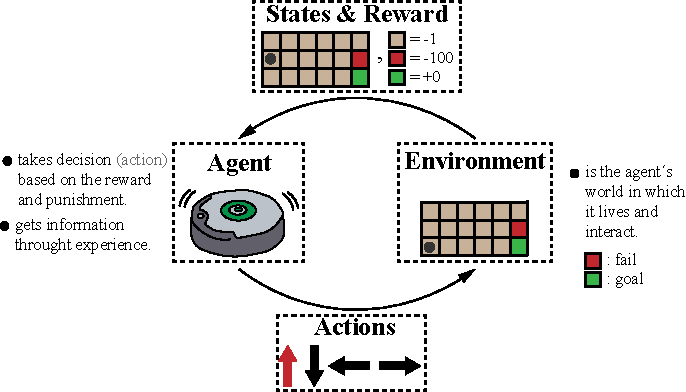
\includegraphics{reinforcement_learning_diagram.pdf}
			\onslide<2>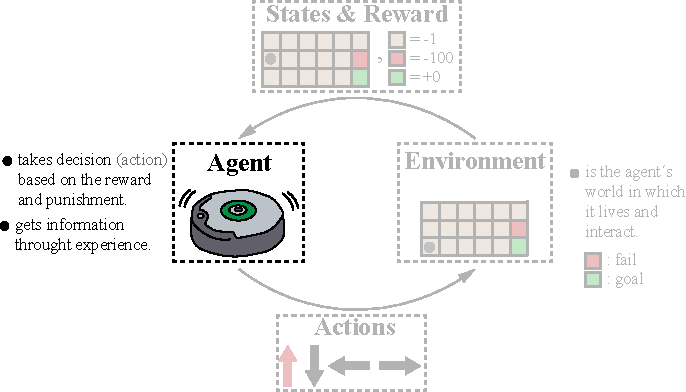
\includegraphics{reinforcement_learning_diagram_1.pdf}
			\onslide<3>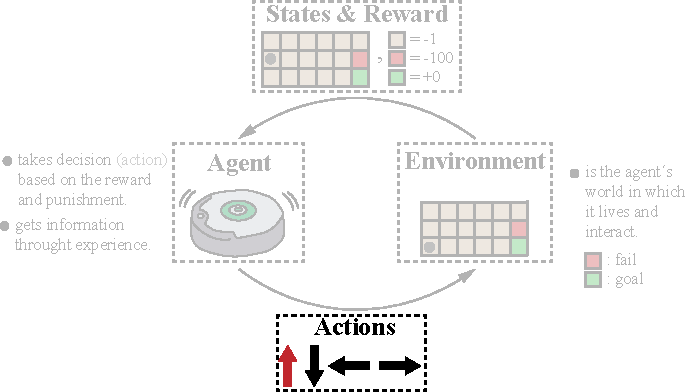
\includegraphics{reinforcement_learning_diagram_2.pdf}
			\onslide<4>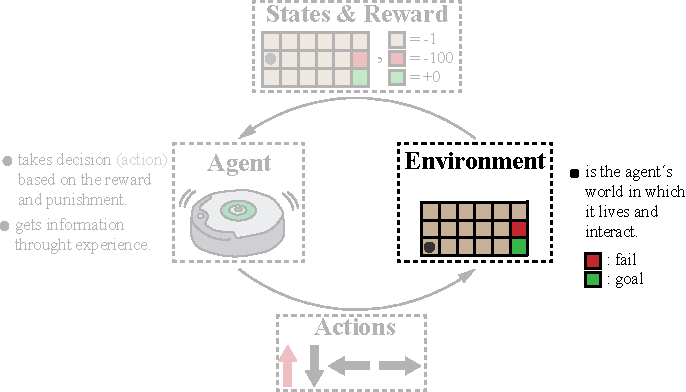
\includegraphics{reinforcement_learning_diagram_3.pdf}
			\onslide<5>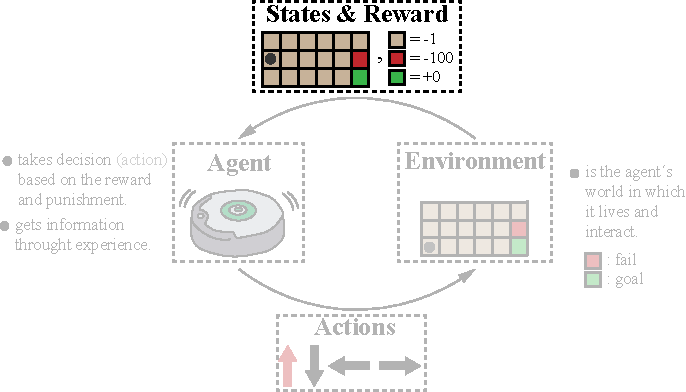
\includegraphics{reinforcement_learning_diagram_4.pdf}
			\onslide<6>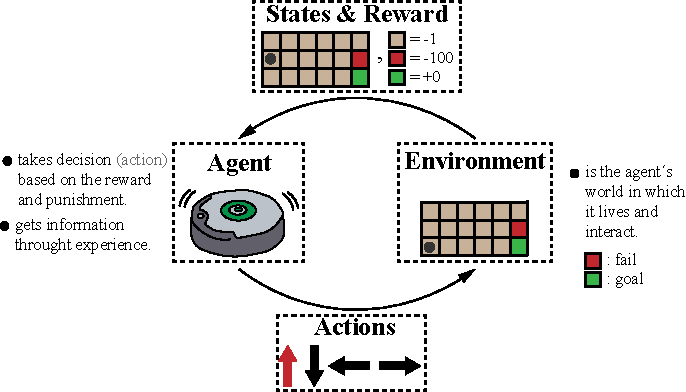
\includegraphics{reinforcement_learning_diagram.pdf}
		\end{overprint}
	\end{figure}

	\footnotetext[1]{R. S. Sutton (2018).}
\end{frame}


\begin{frame}
	\frametitle{Policy}
	A policy ($\pi$) indicates the decision {\color{gray} (action)} that the agent should take as a function of the agent's state to accomplish the task\footnotemark[1].% ($\pi (a|s)$).
	
	\begin{figure}
		\begin{overprint}
			\onslide<1>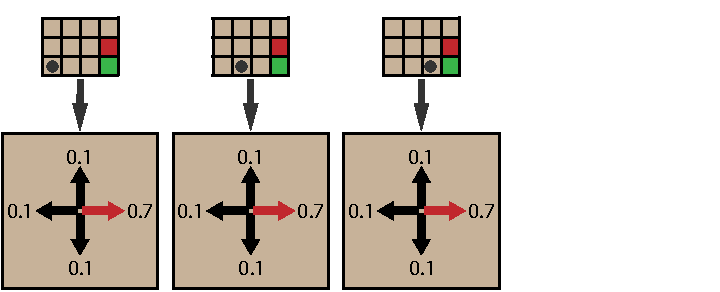
\includegraphics{policy_stochastic_1.pdf}
			\onslide<2>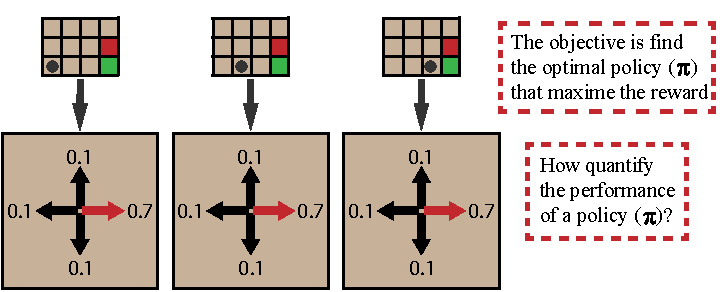
\includegraphics{policy_stochastic.pdf}
		\end{overprint}
		
	\end{figure}
	
	\footnotetext[1]{R. S. Sutton (2018).}
\end{frame}



\begin{frame}
	\frametitle{Policy evaluation: value function}
	% trainning process:  throught experience
	% what happend if I take this action?
	% V^{\pi} indicates the value of a policy
	The value function ($V^{\pi}(s)$) indicates the final return from being in a state when following a particular policy ($\pi$)\footnotemark[1]. It is given by
	\begin{equation*}
		V^{\pi}(s_t= s) = E_{\pi}  \left[r_t + \gamma r_{t+1} + \gamma^{2} r_{t+2}+ . . . | s_t = s \right],
	\end{equation*}
	\noindent where $\gamma$ is a discount factor and $s_t$ is initial state.
	
	\begin{figure}
		\begin{overprint}
			\onslide<1>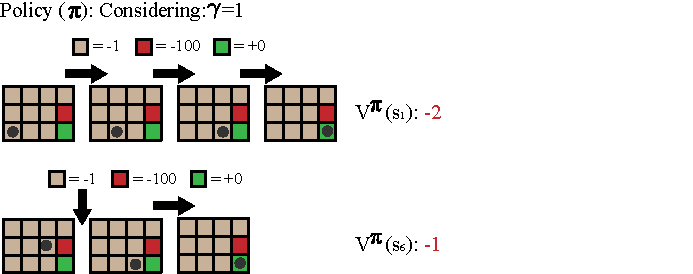
\includegraphics{policy_selection_v3_1.pdf}
			\onslide<2>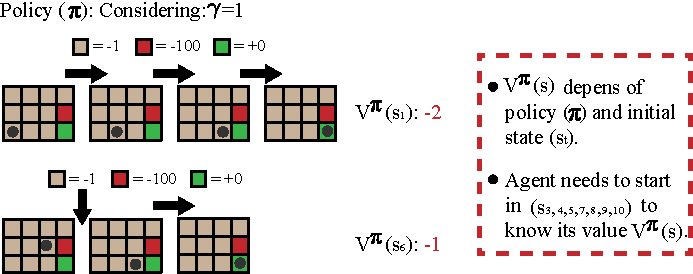
\includegraphics{policy_selection_v3.pdf}
		\end{overprint}
	\end{figure}

	\footnotetext[1]{R. S. Sutton (2018).}
\end{frame}

\begin{frame}
	\frametitle{Value function approximation}
	The value function could be approximated by a neural network

	\begin{figure}
		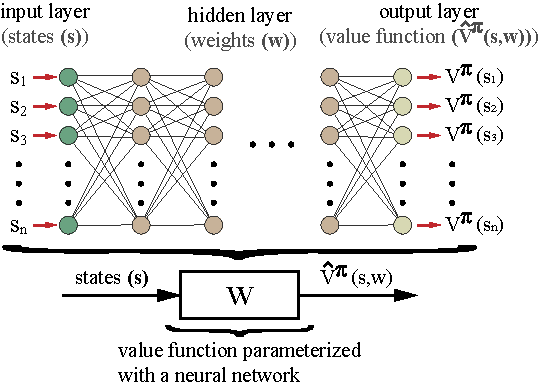
\includegraphics{value_function_cnn.pdf}
	\end{figure}
	
\end{frame}

\begin{frame}
	\frametitle{Policy and neural networks}
	% algorithm to train policy
	% connection between cost function with interesent values 
	
	% a problem of RL is that depends of the trainning data that it generates rather than relyin in static dataset, sometimes could be unstable 
	The policy could be represented by a neural network

	\begin{figure}
		\centering
		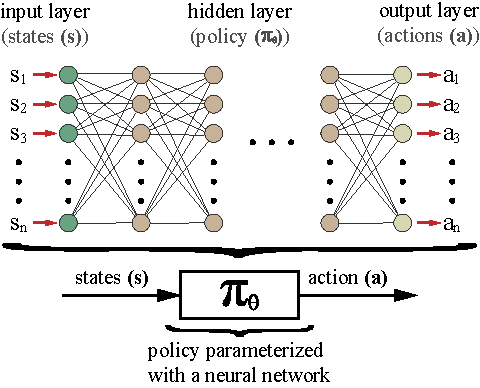
\includegraphics{policy_cnn.pdf}
	\end{figure}

\end{frame}

\begin{frame}
	\frametitle{Policy gradient method}
	This method is focused on modify the neural network parameters  ($\theta$) to get a optimal {\color{gray} (local)} policy\footnotemark[1].

	\begin{center}
		\begin{minipage}{8cm}
			\begin{myexampleblock}[8cm]{}
				The objective function {\color{gray} (reward)} is formulated as\footnotemark[1]				
				\begin{equation*}
					L(\theta) = \expectation \left[ \mathrm{log} \pi_\theta (a|s) \advantage  \right],			
				\end{equation*}
				with,
				\begin{equation*}
					\advantage = V^{\pi_{\theta}}_{t}  - \hat{V}_{t}, 
				\end{equation*}
				where,
				\newline
				\hspace{10px}\makebox[\linewidth][l]{				
				\begin{tabular}{l l}
					${\color{forestgreen} \bullet}$ $\advantage$ & advantage function \\
					${\color{forestgreen} \bullet}$ $V^{\pi_{\theta}}_{t}$ & final reward following policy $(\pi_\theta)$ \\
					${\color{forestgreen} \bullet}$ $\hat{V}_{t}$ & expected final reward {\color{gray}(baseline)}
				\end{tabular}
			 	}
			\end{myexampleblock}
		\end{minipage}
	\end{center}
	\footnotetext[1]{R. S. Sutton (2018).}
\end{frame}

\begin{frame}
	\frametitle{Proximal policy optimization}
	% goal is to find a policy with highest value function V
	% focus on policy gradient methods
	
	PPO is one of the best algorithms for reinforcement learning due to simplicity and high performance\footnotemark[1].
	
	\begin{center}
		\begin{minipage}{9cm}
			\begin{myexampleblock}[9cm]{}
				The main objective function {\color{gray} (reward)} is given by
				\begin{equation*}
					L^{\mathrm{CLIP}}(\theta) = \expectation \left[ \mathrm{min} \left(  r_{t}(\theta)  \advantage,  \mathrm{clip} (r_{t}(\theta) , 1-\epsilon, 1+\epsilon) \advantage  \right)  \right],			
				\end{equation*}	
				with,
				\begin{equation*}
					r_{t}(\theta) =\ratio,
				\end{equation*}
				where,
				\newline
				\hspace{10px}\makebox[\linewidth][l]{	
					\begin{tabular}{l l}
						${\color{forestgreen} \bullet}$  $r_{t}(\theta)$ & probability ratio between policies 
						\\
						${\color{forestgreen} \bullet}$ $\epsilon$ &  hyperparameter
					\end{tabular}		
				}
			\end{myexampleblock}
		\end{minipage}
	\end{center}
	
	\footnotetext[1]{J. Schulman (2017).}	
\end{frame}

\begin{frame}
	\frametitle{Proximal policy optimization}
	\begin{figure}
		\centering
		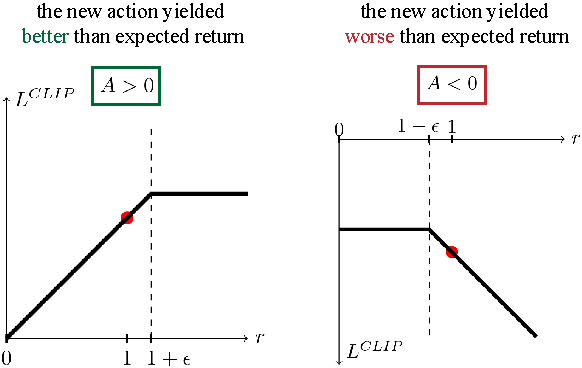
\includegraphics{advantage.pdf}
		\caption{Image adapted from J. Schulman (2017)}
	\end{figure}
	
\end{frame}

\begin{frame}
	\frametitle{Proximal policy optimization}
	% goal is to find a policy with highest value function V
	% focus on policy gradient methods	
	\begin{center}
		\begin{minipage}{10cm}
			\begin{myexampleblock}[10cm]{}
				The final objective function {\color{gray} (reward and exploration)} is given by\footnotemark[1]
				\begin{equation*}
					L^{\mathrm{PPO}}(\theta) = \expectation \left[  L^{\mathrm{CLIP}}(\theta) - c_1 L^{\mathrm{VF}}(\theta)  + c_2 S[\pi_\theta](s_t)  \right],			
				\end{equation*}	
				with,
				\begin{equation*}
					L^{\mathrm{VF}}(\theta) = \left( V_\theta (s_t) - V^{\mathrm{target}}_{t}  \right)^{2},
				\end{equation*}			
				where,
				\newline
				\hspace{10px}\makebox[\linewidth][l]{	
					\begin{tabular}{l l}
						${\color{forestgreen} \bullet}$  $c_1$, $c_2$ & weighting coefficients \\
						${\color{forestgreen} \bullet}$ $S$ & entropy bonus {\color{gray} (exploration)} \\
						${\color{forestgreen} \bullet}$  $ L^{\mathrm{VF}}(\theta)$ & square-error loss \\
						${\color{forestgreen} \bullet}$ $V^{\mathrm{target}}_{t}$ & objective final reward
					\end{tabular}		
				}
			\end{myexampleblock}
		\end{minipage}
	\end{center}
	
	\footnotetext[1]{J. Schulman (2017).}	
\end{frame}

\begin{frame}
	\frametitle{Simulation environment and libraries}

		\begin{columns}
			\begin{column}{.5\textwidth}
				\begin{figure}
				\centering
				
\includegraphics[width=0.9\textwidth]{mujoco_logo.pdf}
				\end{figure}
				\vspace{20px}
				\begin{figure}
					\centering
					
\includegraphics[width=0.8\textwidth]{openAI_logo.pdf}
				\end{figure}
				%\caption{Spring-loaded inverted pendulum (SLIP)}				
			\end{column}
			\begin{column}{.5\textwidth}
				\begin{figure}
				\centering
				
\includegraphics[width=0.7\textwidth]{tensorflow.pdf} 
				\end{figure}
				%\caption{New model with three segment leg}				
			\end{column}
		\end{columns}	
	
\end{frame}

\begin{frame}
	\frametitle{Bipedal robot: algorithm configuration}
	
	\begin{columns}
	\begin{column}{.5\textwidth}
	\begin{figure}
		\centering
		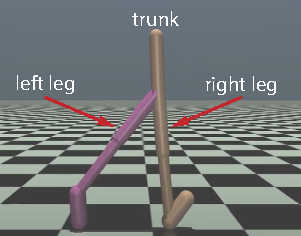
\includegraphics{bipedal_robot.pdf}
		\caption{Bipedal robot in simulation environment}
	\end{figure}
	\end{column}
	
	\begin{column}{.5\textwidth}
			\begin{exampleblock}{States}
				\begin{itemize}
					\item position: $6$ (left, right) $+$ $1$ (trunk)
					\item velocity: $6$ (left, right) $+$ $1$ (trunk)
					\item total: $14$ states
				\end{itemize}
			\end{exampleblock}

			\begin{exampleblock}{Reward}
				\begin{itemize}
					\item fail when trunk angle $>$ $50^{\circ}$
					\item $+1$ for each iteration alive
					\item $+$ linear velocity
				\end{itemize}
				
			\end{exampleblock}		
	\end{column}
	\end{columns}
\end{frame}


